\chapter{Results}

The data clearly show first a relationship between cell state of charge the acoustic TOF through the cell, then between induced lithium plating and changes in acoustic time of flight data, and finally between changes in ambient temperature and change in acoustic TOF through the cell. 

Recall that the three sources of change in acoustic time of flight through a cell are change in state of charge, change in state of health, and change in ambient conditions. 
By systematically adding and understanding changes in each category to the experimental conditions, shifts in acoustic ToF through the cell can be observed, analyzed, and then attributed to each source of change.

When the ambient conditions were steady, the relationship between SoC and ToF was very clear \todo{plot}. Ambient temperature variation clearly has a significant effect on the acoustic TOF shifts. \todo{fig} shows a comparison between the measured TOF data and "idealized" TOF from a gentle, non-plating routine, constructed by assuming the data ought not change between cycles and copying the first waveform repeatedly as a result. In the absence of plating and at the same state of charge, the relationship between change in ToF shift and change in ambient temperature is consistent enough that much of the influence of temperature can be scrubbed out using simple regressions.

\section{Time of Flight Shift Due to Change in State of Charge}
The data clearly demonstrate a strong and consistent relationship between acoustic ToF through the cell and the cell's state of charge while ambient conditions and cell state of health are held steady.

The shift in ToF was determined using a colleague's cross-correlation analysis of each received waveform to a reference waveform. The reference waveform was chosen from one of earliest waveforms in the experiment, but not too early, in order to allow for start-up effects to dissipate.
During the C/2.5 charge and discharge cycling, which does not appreciably plate the cell and therefore can be assumed to not change the state of health of the cell, the ToF data follows a very regular pattern. 
The ToF shift peaks at roughly the same value, and at the same point in the cycling protocol: when the routine finishes charging. 
Conversely, the ToF shift experiences a minimum of fairly consistent value at the end of each discharge period.

\todo{fig}

\section{Time of Flight Shift Due to Change in State of Health}
The data in the same test goes on to demonstrate acoustic TOF analysis's capability to observe plating, and therefore change in a cell's state of health. This is shown during the 5C and especially 10C routines in the experiment. 
While the TOF data maintains a consistent form for each of those protocols, the "neutral axis" to which it returns between cycles increases each time. 
Since the ambient conditions were steady and there was no variation in the cycling protocols, these changes in the TOF shift show lingering changes in the state of health of the cell. 
This is corroborated in each of the experiments. 
SEM (scanning electron microscope) and XPS (X-Ray Photoelectron Spectroscopy) analysis confirm plating on the electrodes of the cells, but such techniques do not provide information on when the plating occurred. \todo{moar}

To confirm plating had indeed occurred, a cell was dissected and used for optical, SEM, and XPS analysis.

\begin{figure}[t]\label{fig:optical}
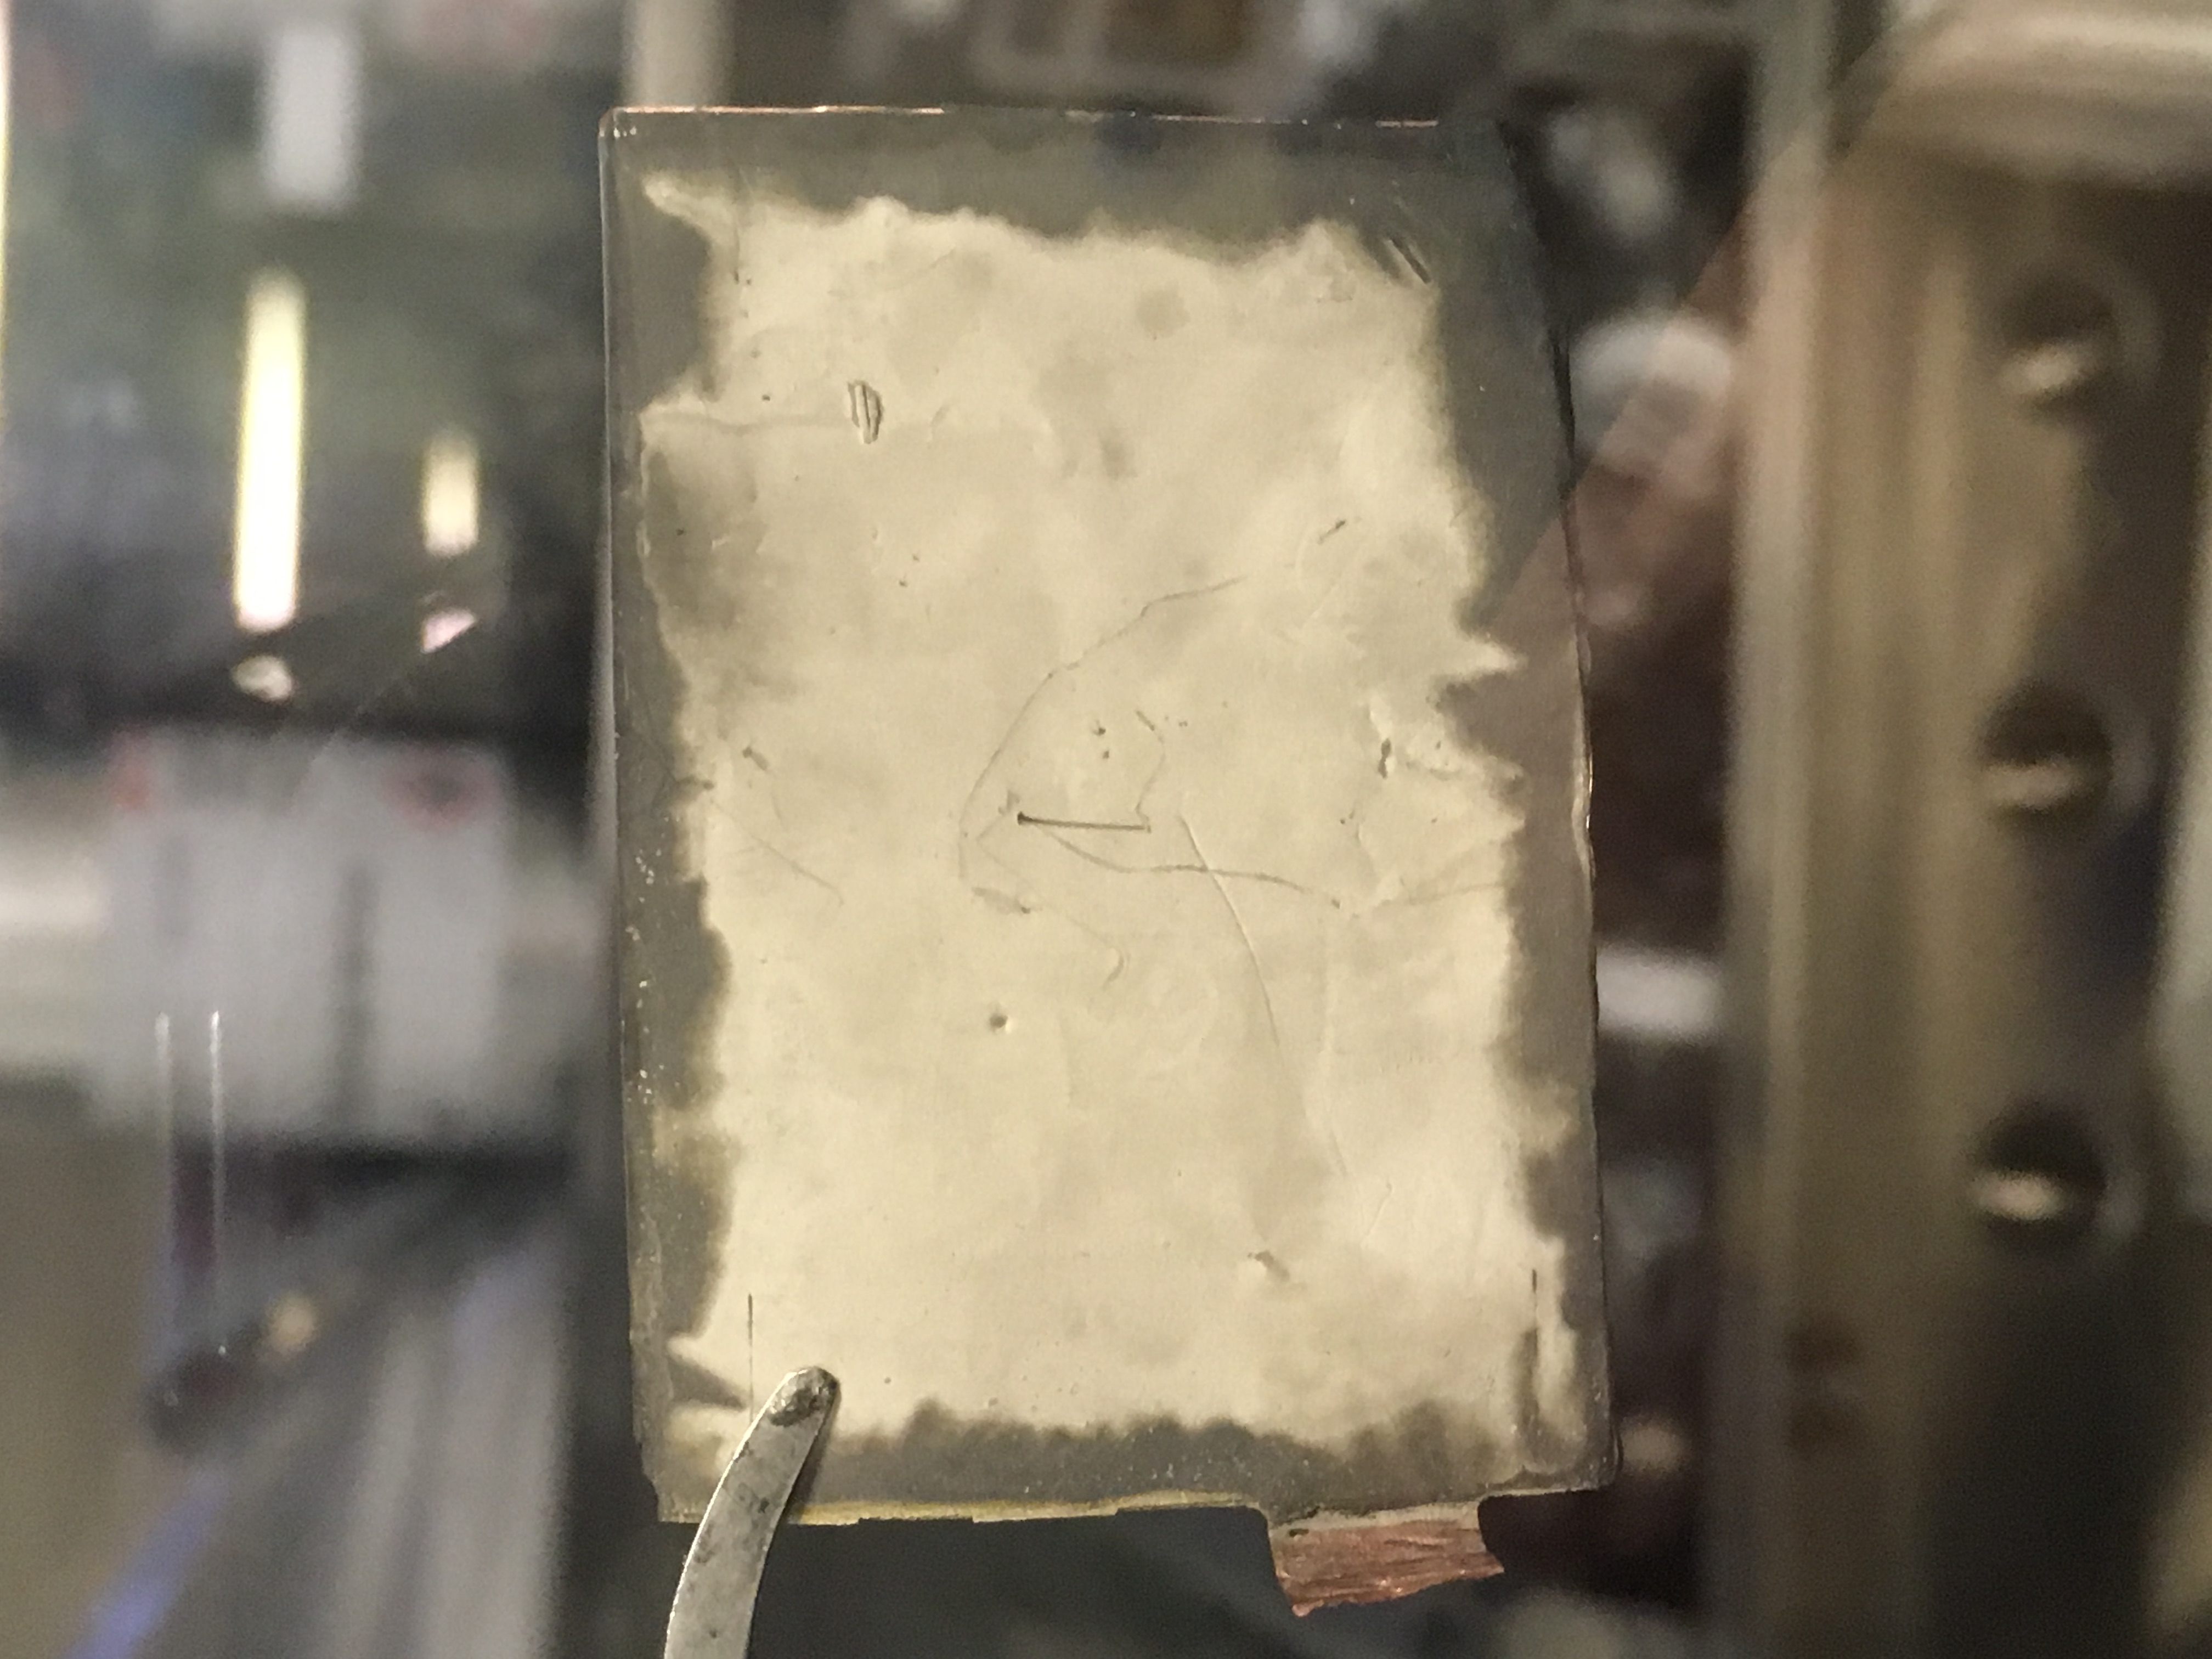
\includegraphics[width=0.6\textwidth]{Thesis/optical.JPG}
\centering
\caption{A cell cut open after electrochemical cycling. The light region is lithiated.}
\end{figure}

Optical analysis provided quick confirmation that the cell had plated; since the cell had not been used before the experimental protocol described above, it can be safely assumed the plating occurred then. SEM and XPS analyses provide more sophisticated information about the plating. 

\section{Time of Flight Shift Due to Change in Ambient Conditions}
In the first experiment which demonstrated the technique, ambient temperature was held quite steady, and had no material impact on acoustic TOF through the cell. 
However, subsequent experiments were unable to maintain such optimal conditions.
During routines using gentle C/2.5 cycling, thus maintaining state of health, the influence of ambient temperature changes on acoustic TOF can be isolated from the influence of state of charge changes with reasonable success. 
Polynomial fits and linear regressions correlate change in ambient temperature with change in ToF shift. 

The thermocouples and transducers have different sampling rates and schedules, so a couple approaches created paired change in ToF shift and change in temperature data; these are plotted against each other in \todo{ref}. 
In one version of the analysis, change in temperature data was averaged across a cycle and regressed against change in TOF shift data. 
More accurate results resulted from interpolating the temperature data using linear or polynomial fits, depending on the shape of the temperature data.

The analysis shows a reasonable estimate at how the ToF would shift without the influence of the ambient temperature shifts, potentially broadening the application of the technique in monitoring cells.
\begin{figure}[t]\label{fig:0417tofshiftadj}
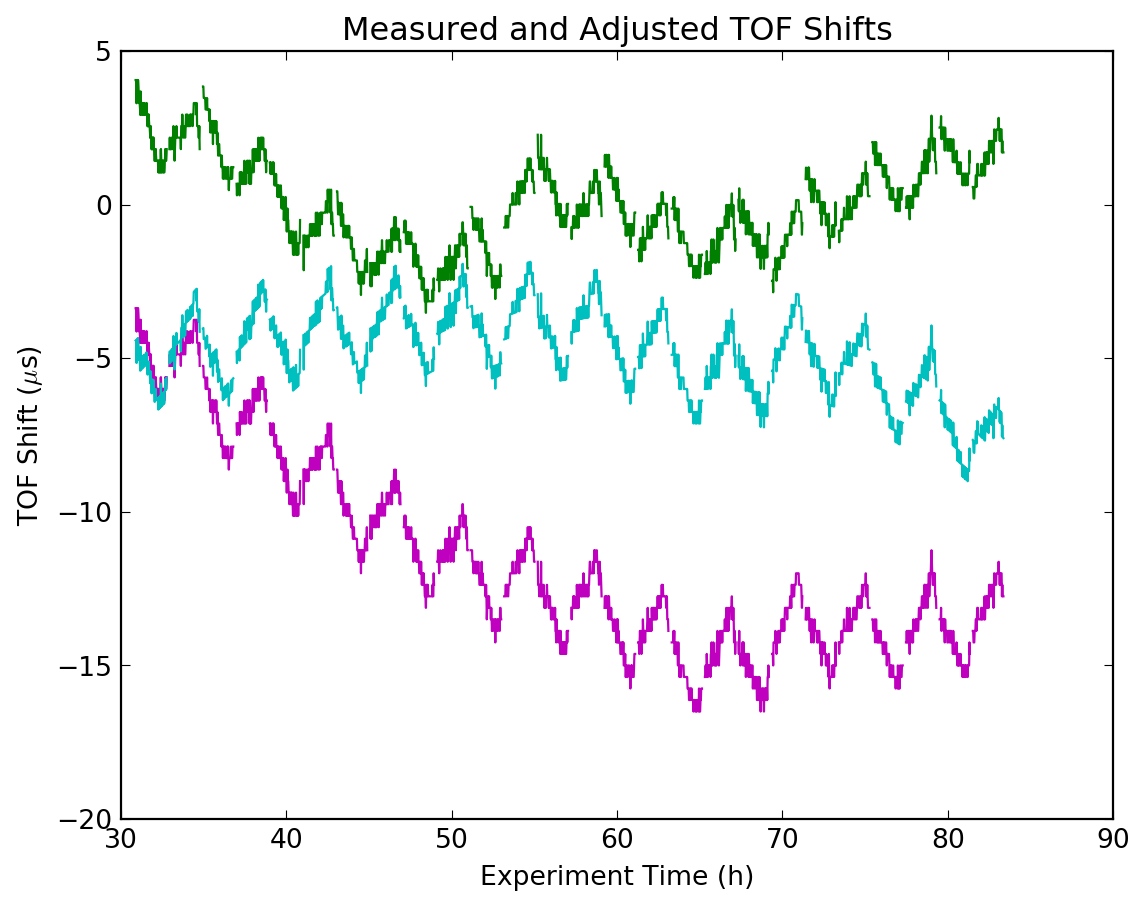
\includegraphics[width=0.75\textwidth]{Thesis/0417tofshiftadj.png}
\centering
\caption{ToF Shift across the experiment. This plot compares the unaltered ToF shift, the ToF shift adjusted using a change in ToF - change in temperature regression using interpolated temperatures, and the ToF shift adjusted using a regression of maximum change in ToF shifts and averaged temperatures.}
\end{figure}

One check is to compare them to an idealized prediction of how the TOF should actually shift during the experiment. 
Since each cycle at a particular charge rate has a consistent duration and consistent effect on the cell's state of charge, it is easy to compare ToF shift data between cycles. 
At any particular point in the cycle's duration, the ToF shift in each cycle should match. Charge and discharge cycle ToF data, when overlaid (see \hyperref[fig:0417overlays]{\cref{fig:0417overlays}}), show how consistent or inconsistent the ToF shifts are across the experiment.
Ideally there would be perfect overlap in the data from each cycle within a protocol within an experiment, but before the ambient temperature shift's influence was removed, this was clearly not the case. 
The overlap is still imperfect after the TOF shift data was adjusted based on the regressions, but it is much better.

\begin{figure}[t]\label{fig:0417overlays}
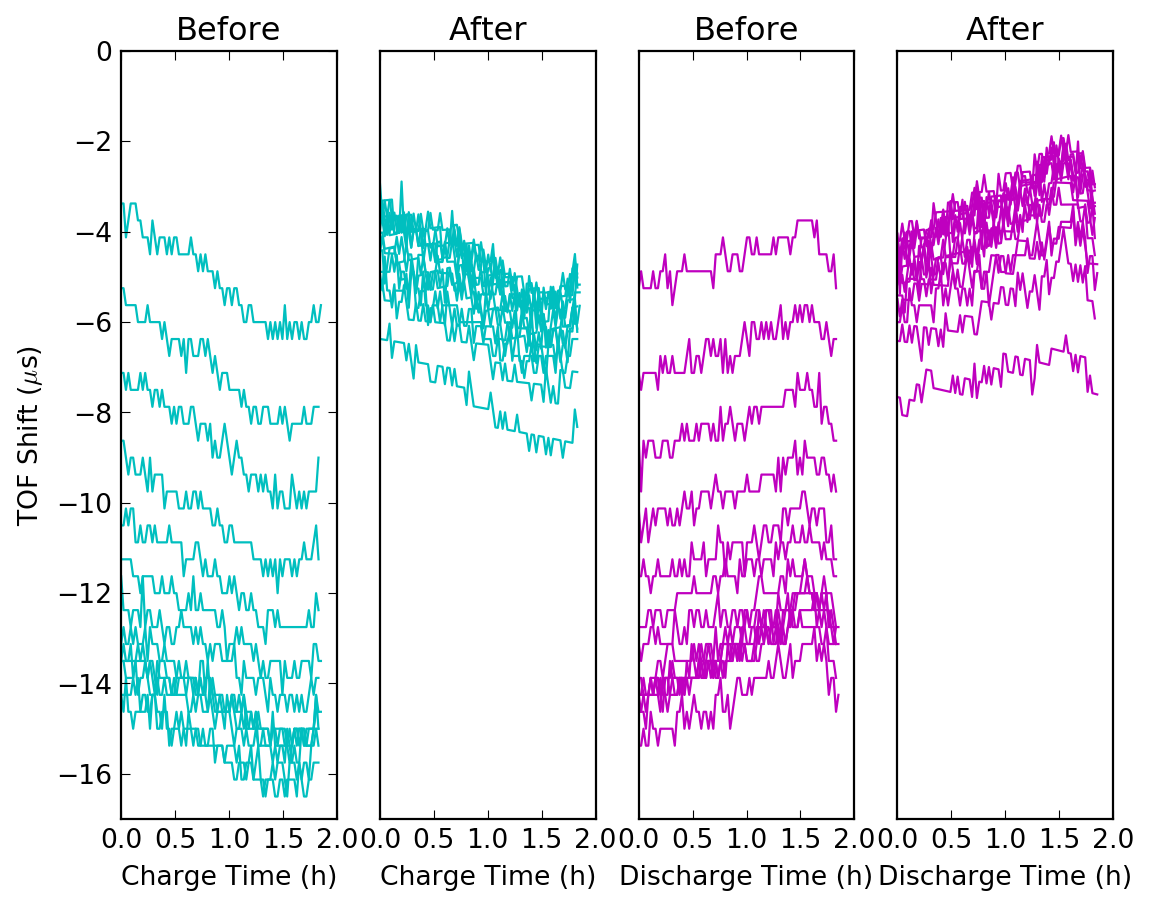
\includegraphics[width=0.95\textwidth]{Thesis/0417overlays.png}
\centering
\caption{Overlays of the raw and adjusted ToF shifts across each charge cycle (far and center left) and discharge cycle (center and far right). The adjusted data used a regression to remove the influence of ambient temperature fluctuations.}
\end{figure}
